\documentclass{webofc}
\usepackage[varg]{txfonts}   % Web of Conferences font

\usepackage{listings}
\usepackage{minted}
\usepackage{subfig}
\usepackage{hyperref}
\usepackage{graphicx}
\usepackage{subcaption}
\usepackage{tikz}

\usepackage[varg]{txfonts}   % Web of Conferences font

\newminted{cpp}{gobble=2, numbersep=3pt, escapeinside=||, xleftmargin=8mm, framesep=2mm, frame=leftline, baselinestretch=1, fontsize=\scriptsize, linenos=true}
\newmintinline{cpp}{}

\usetikzlibrary{shadows, arrows, fit, positioning, matrix, shapes}
\usetikzlibrary{decorations.markings}

% Define colors
\definecolor{my_yellow}{RGB}{255, 253, 217}
\definecolor{my_orange}{RGB}{255, 127, 0}
\definecolor{my_lightblue}{RGB}{105, 186, 249}
\definecolor{my_purple}{RGB}{150, 154, 219}
\definecolor{my_green}{RGB}{90, 194, 160}

% Define block styles  
\tikzset {
  bigbox/.style = {draw, thick, fill=gray!10, rounded corners, rectangle},
  box/.style = {draw, thick, minimum height=0.8cm, minimum width=1.5cm, rounded corners, rectangle, fill=white, anchor=south},
  model/.style = {draw, thick, fill=white, text centered, minimum height=3em, minimum width=4em, rounded corners, drop shadow},
  user/.style = {draw, thick, ellipse, fill=white, text centered, minimum height=3em, minimum width=5em, drop shadow},
  line/.style = {->, thick, color=black, shorten <=2pt, shorten >=2pt, >=stealth'},
  dashed/.style = {->, dash pattern=on 3pt off 3pt, color=gray, shorten <=2pt, shorten >=2pt, >=stealth'},
  plain/.style = {minimum width=1em},
  %\draw [line, ->] (m1.north) ++(-15pt,-1pt) arc [start angle=-140, end angle=-400, radius=20pt] node[midway] {$T_{M_1}$} ;
  % This works around an issue with node[midway] http://tex.stackexchange.com/questions/38763/how-to-place-a-node-in-the-middle-of-an-arc                
  arcnode/.style 2 args={
    decoration={
                 raise=#1,             
                 markings,   
                 mark=at position 0.5 with {\node[inner sep=0] {#2};}
            },
            postaction={decorate}
    }
}

% Define the layers to draw the diagram
\pgfdeclarelayer{background}
\pgfdeclarelayer{foreground}
\pgfsetlayers{background,main,foreground}

% Draw background
\newcommand{\background}[5]{%
  \begin{pgfonlayer}{background}
    % Left-top corner of the background rectangle
    \path (#1.west |- #2.north)+(-0.5,0.25) node (a1) {};
    % Right-bottom corner of the background rectanle
    \path (#3.east |- #4.south)+(+0.5,-0.25) node (a2) {};
    % Draw the background
    \path[rounded corners, draw=black!50, dashed, name=box]
      (a1) rectangle (a2);
    \path (a1 |- a2) -- (a2) node[midway,below] {\large\textit{#5}};
  \end{pgfonlayer}}

% Define a circled symbol command used throughout the thesis.
\newcommand*\circled[1]{\tikz[baseline=(char.base)]{
            \node[shape=circle,draw,inner sep=2pt] (char) {#1};}}
            

\begin{document}
%
\title{Continuous Performance Benchmarking Framework for ROOT}
%
% subtitle is optionnal
%
%%%\subtitle{Do you have a subtitle?\\ If so, write it here}

\author{\firstname{Oksana} \lastname{Shadura}\inst{1}\fnsep\thanks{\email{oksana.shadura@cern.ch}} \and
        \firstname{Vassil} \lastname{Vassilev}\inst{2}\fnsep\thanks{\email{vvasilev@cern.ch}}
        \firstname{Brian Paul} \lastname{Bockelman}\inst{1}\fnsep\thanks{\email{bbockelm@cse.unl.edu}}
}

\institute{University of Nebraska Lincoln, 1400 R St, Lincoln, c, United States
\and
           Princeton University, Princeton, New Jersey 08544, United States
          }
\abstract{%
  
Foundational software libraries such as ROOT are under intense pressure to avoid software regression, including performance regressions. Continuous performance benchmarking, as a part of continuous integration and other code quality testing, is an industry best-practice to understand how the performance of a software product evolves over time. We present a framework, built from industry best practices and tools, to help to understand ROOT code performance and monitor the efficiency of the code for a several processor architectures. It additionally allows historical performance measurements for ROOT I/O, vectorization and parallelization sub-systems.

%We utilize the Google benchmarking library to execute micro benchmarks of selected hotspot functions in ROOT and related libraries. This provides detailed data measurements, including memory usage and CPU instruction counters. Additionally, the framework manages traditional benchmarking pitfalls via repeating unstable benchmarks and providing a stable performance environment over time. The performance data points from continuous benchmarking are fed into an InfluxDB database and provided to the developer community via a Grafana-based dashboard. This performance benchmarking framework, built on generic and flexible infrastructure, is meant to be reusable by other projects.

}
%
\maketitle
%
\section{Introduction}

Last decade software development has grown in size and complexity. Industry best practices include extensive quality testing on different levels based on time intervals or before a change is accepted. Regular quality assurance in the process of software development is widely known as continuous integration. Continuous integration relies on various kinds of tests and mainly focuses on finding incorrect behavior. Quite often, correct behavior is defined pragmatically to assume that for certain input data there shall be certain expected output data. In some domains, however, non-scalable (or non-performant) correct behavior can be as devastating as incorrect behavior. Extending the definition of correct behavior to include performance metrics is a challenging but rewording task.

Performance is essential for the field of high-energy physics (HEP) and in particular its core libraries such as ROOT. The LHC Run 3 era promises to make no compromise on every bit of performance and performance regressions may be classified as critical for experiments' software stacks. Metrics such as threading scalability or vectorization level are already becoming a necessity.

On one hand, performance becomes fundamental for software toolchains in HEP. On the other hand, performance analysis is still a laborious job which requires expertise. Reasoning about performance is hard as it may require different (expensive or not-available) hardware, running with multiple compilers on different platforms or experimenting with specific setups. We believe, much of the work can be automatized to show performance by-products in the forms of diagrams accessible to non-experts. This paper discusses challenges of developing a continuous \textit{performance} monitoring system for ROOT; argues for the need of small-scale benchmarks; and discusses ways to visualize the obtained data. More concretely, we describe the \textit{ROOTBench} system providing:
\begin{itemize}
\item an extensible system tracking different performance metrics of the facilities in ROOT;
\item speculative performance evaluation of proposed changes;
\item rich and customizable visualizations and aids for performance analysis.
\end{itemize}

This paper is structured as follows: Section 1 (Introduction); Section 2 (Background); Section 3 (Information Flow in ROOTBench); Section 4 (Usage of ROOTBench); Section 5 (Results); and Section 6 (Conclusion).
 
\section{Background}

The requirements for the designed system are in three main categories: performance monitoring primitives, visualization features and data storage. The performance monitoring system should have at least facilities for measuring elapsed time, memory footprint and user-defined counters. It should have a way to stabilize the results among runs and should have primitives for preventing compiler optimization for particular pieces of code if the user needs them. The visualization should happen on the web and users should be able to define custom dashboards. The database should have time-series as a first class citizen to enable easy browsing and comparisons of historical data.

We will make a brief overview of Google benchmark library \cite{gbench}, Celero \cite{celero}, Nonius \cite{nonius} and hayai \cite{hayai} which are framework fulfill to some of all of the requirements. Nonius is a small open-source framework for benchmarking small parts of C++ code, inspired by Criterion, a similar Haskell-based tool. Celero, Nonius, hayai have smaller community with not clear perspective of continuous support of products. Google benchmark is developed by Google and supported by a wider community.

Googlebench \cite{gbench} is C++ library, inspired by googletest and the xUnit architecture.  This library is lightweight and supports different type benchmarks: both value- and type-parameterized. Google benchmark also provides various options for running the benchmarks including multithreading, and custom report generation.


A key ingredient for benchmarking infrastructure is modern visualization tool, that will require minimal maintenance efforts. Visualizing data helps monitor performance of ROOT, detect patterns and take an action when identifying anomalous behavior. There are significant amount of data visualization tools, used for operations with collected data logs and measurements. We will focus on the most popular and competitive products: Kibana \cite{kibana} and Grafana \cite{grafana}.

Kibana is an open source, browser-based analytics and search dashboard for Elasticsearch \cite{elasticsearch}. Kibana has very good learning curve and it is flexible and powerful. Grafana is a general purpose dashboard and graph composer. It is focused on providing rich ways to visualize time series metrics, mainly though graphs but supports other ways to visualize data through a plugin panels. It currently has rich support for for Graphite, InfluxDB and OpenTSDB and it supports other data sources via plugins. General purpose of Grafana makes it ideal candidate for ROOT performance infrastructure. Both platforms have similar feature sets.

We decided to utilize the Google benchmarking library because it gives good control over hotspot functions in ROOT and related libraries. This provides detailed data measurements, including memory usage and CPU instruction counters. Additionally, the framework manages traditional benchmarking pitfalls via repeating unstable benchmarks and providing a stable performance environment over time. Last but not the least, it has compatible license with ROOT and backed up by major industry company.

We chose the Grafana because of the offered feature set and because CERN provides first class service for it. In turn, this selects InfluxDB as our time series database because of the native support in Grafana. The setup helps to store a sequence of measured data points, providing data for the same performance measurements over time and stored in time order or as series of numeric values. Each of measurements is paired with a timestamp, defined by a name and a set of labeled dimensions (or “tags”).


%Performance benchmarking is essential part of the software development especially for experiment software stacks, that required to become more scalable, fast and efficient for upcoming LHC Run 3. 
%One of the challenging tasks is to be able to monitor performance correctness. Taking in account factors, such as operation system, system library updates, changes in standard library or compiler upgrade that could cause performance measurements changes or "bumps "in benchmarks measurements, we decided to run benchmarks on dedicated physical machine. Benchmarks are always launched in the same conditions like in a sequential mode, taking into account the noise coming from system processes (updates etc.). Our goal is provide reliable and trustable results to end users.

%ROOT performance benchmarking is helping to bring to the light hotspots of vectorization, concurrency and other crucial performance components and track  performance of newly introduced technologies in ROOT (e.g. runtime C++ modules (LINK)). In current status of integration, benchmarks are hosted in rootbench.git \cite{rootbench}. Integration with ROOT helps capturing performance statistics and it is mostly making sure tests pass (i.e. checks correctness).


\section{Information Flow in ROOTBench}

ROOTBench is built from industry best practices and tools, to help understand ROOT code performance and monitor the efficiency of the code for a several processor architectures. It additionally allows historical performance measurements for ROOT I/O, vectorization and parallelization sub-systems.

\begin{figure}[!h]
  \centering
  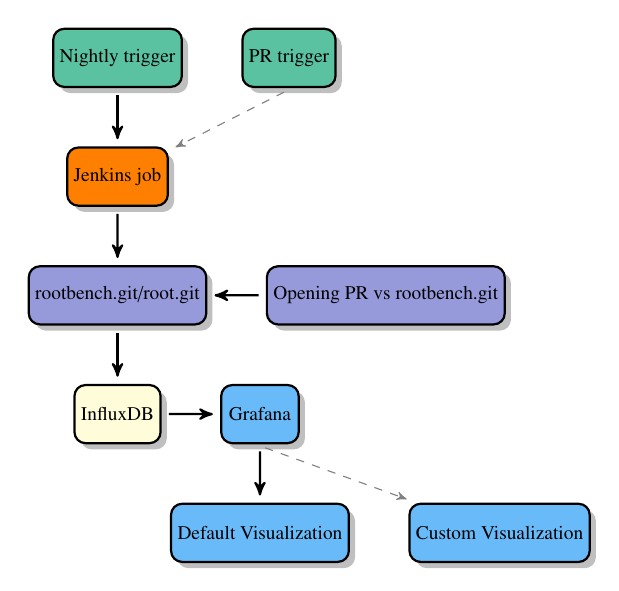
\begin{tikzpicture}[outer sep=0.05cm, node distance=0.8cm, scale=0.7, transform shape]
        
    \node[model, fill=my_green, name=nt] (nt) {Nightly trigger};
    \node[model, fill=my_green, name=pr, right=1cm of nt] (pr) {PR trigger};
    \node[model, fill=my_orange, name=jj, below=1cm of nt] (jj) {Jenkins job};
    \node[model, fill=my_purple, name=git, below=1cm of jj] (git) {rootbench.git/root.git};
    \node[model, fill=my_purple, name=gitpr, right=1cm of git] (gitpr) {Opening PR vs rootbench.git};
    \node[model, fill=my_yellow, name=influxdb, below=1cm of git] (influxdb) {InfluxDB};
    \node[model, fill=my_lightblue, name=grafana, right=1cm of influxdb] (grafana) {Grafana};
    \node[model, fill=my_lightblue, name=def_vis, below=1cm of grafana] (def_vis) {Default Visualization};
     \node[model, fill=my_lightblue, name=custom_vis, right=1cm of def_vis] (custom_vis) {Custom Visualization};

    \draw[line, ->] (nt.south) -- (jj);
    \draw[dashed, ->] (pr.south) -- (jj);
    \draw[line, ->] (jj.south) -- (git);
    \draw[line, ->] (gitpr) -- (git);
    \draw[line, ->] (git.south) -- (influxdb);
    \draw[line, ->] (influxdb.east) -- (grafana);
    \draw[line, ->] (grafana.south) -- (def_vis);
    \draw[dashed, ->] (grafana.south) -- (custom_vis);

  \end{tikzpicture}
  \caption{Jenkins -- ROOTBench Flow.}
  \label{fig:InformationFlow}
\end{figure}

The information flow of system starts from a user-defined benchmark. It is written using the Google benchmark framework and compiled to a standalone executable. All benchmark executables are compiled by a Jenkins job every night. This happens by building the ROOT framework and building ROOTbench (rootbench.git) repository against it. After building we run the set of benchmarks in sequential mode on a dedicated machine to reduce the performance fluctuations as much as possible. After each benchmark, the performance data points from continuous benchmarking are fed into an InfluxDB database.

The system is decoupled as shown in Fig~\ref{fig:InformationFlow}. Grafana, reads the database and visualizes the obtained data, making it public to the developer community via various Grafana dashboards. Our framework is built on generic and flexible infrastructure and can be reused for other projects easily. The tool can be connected to Jenkins or other similar services. We utilize special Jenkins jobs triggered on nightly basis.


%\begin{figure}
%\includegraphics[width=1.0\linewidth]{pictures/flow.png}
%\caption{Jenkins -- ROOTBench Flow.}
%\label{fig:InformationFlow}
%\end{figure}

\section {Usage of ROOTbench}


Writing micro benchmarks instead of monolithic macro benchmarks is more relevant for monitoring of performance of software hotspots. Micro benchmarks are hard to write but easy to debug, whereas macro benchmarks are easy to write and hard to debug.

Often, in macro benchmarks where each of the components are contributing to the average performance independently. We can experience problems with hotspots and need of extra profiling with help of such tools as flame graphs or dedicated performance debugging tools such as Intel VTune \cite{vtune}. It helps to find which component is reducing the average performance, with an overhead and extra time invested in investigation of performance bottlenecks of macro benchmark. In addition, macro benchmarks can hide performance regressions because the overall runtime is greater.

The idea of a micro benchmark is to provide a routine which checks performance only for a small set of targeted functionality. In other words, the call stack should be as shallow as possible. The concept of a micro benchmark is similar to the concept of well-written unit test. This kind of benchmarks is very sensitive and can easily amplify and outline regressions. Assuming that we control the system noise well, finding regressions is a lot easier.

It can be challenging for micro benchmarking infrastructure to provide stability of measurements in time, especially for physical machines used for measurements for long times (for getting historical data).  One of requirements is that we need to be able to detect noise from the data and tracking regressions.

\vspace{2em}

We would like to introduce to the reader, in practical terms, how to use the ROOTBench system. We will use two examples checking scalability with respect to vectorisation and threading.

\begin{listing}[h]
    \noindent
    \begin{minipage}[h]{.7\textwidth}
   \begin{cppcode*}{}
  #include <benchmark/benchmark.h>
  #include "Math/GenVector/Transform3D.h"
  #include "Math/Types.h"

  template <typename T>
  static void BM_Plane3D_Hessian(benchmark::State &state) {
     const double a(p0(ggen)), b(p1(ggen)), c(p2(ggen)), d(p3(ggen));
     for (auto _ : state) {
        Plane<T> sc_plane(a, b, c, d);
        sc_plane.HesseDistance();
     }
   }
   BENCHMARK_TEMPLATE(BM_Plane3D_Hessian, double)->Unit(benchmark::kMicrosecond);
   BENCHMARK_TEMPLATE(BM_Plane3D_Hessian, ROOT::Double_v)->Unit(benchmark::kMicrosecond);
   BENCHMARK_MAIN();
   \end{cppcode*}
   \end{minipage}
   \caption{Monitoring vectorization scalability of Plane3D::Hessian}
   \label{vec_bench}
\end{listing}

Listing~\ref{vec_bench} starts by inclusion of the benchmarking primitives and the checked entities. Then we define a function which will monitor the \textit{GenVector}'s \textit{Plane3D::HesseDistance}. After the initialization section we use a loop which is controlled by the framework. It's purpose is to stabilize the results. Next two macro expansions \textit{BENCHMARK\_TEMPLATE} are used for registering our \textit{BM\_Plane3D\_Hessian} as a monitoring function. We register two instances of the function, one taking standard type \textit{double} and a second one taking a vectorization-enabling type \textit{ROOT::Double\_v}. This allows us to compare the level of vectorization against the baseline. We finish by defining the benchmark executable main function via \textit{BENCHMARK\_MAIN}.
%The visualization of a similar to the example function can be seen in Figure~\ref{fig:genvec}. There we also check the scalability with respect to various data loads.

Listing~\ref{thread_bench} defines a multi-threaded benchmark. Line 7, 8, 20 and 21 show the initialization and destruction sections. In the loop we monitor a small helper function which uses the \textit{TBufferMerger} API to fill a \textit{TTree} with random data. Line 11 makes the benchmark configurable by allowing to set the flush level by specifying a \textit{Range} configuration.

The benchmark registration tells the benchmark to use flush rates between 1 and 32 MB with a step of 8. We  configure the benchmark to use real time which is more important in multithreaded environments. In addition we set a thread range in the interval between 1 and twice the number of underlying hardware threads to measure hyperthreading effects. The visualization of a similar to the example function can be seen in Figure~\ref{tbuf}.

\begin{listing}[h]
   \noindent
   \begin{minipage}[h]{.7\textwidth}
   \begin{cppcode*}{}
   // ...
   BufferMerger *Merger = nullptr;
   static void BM_TBufferFile_FillTree(benchmark::State &state) {
      ROOT::EnableThreadSafety();
      using namespace ROOT::Experimental;
      // Setup code here.
      if (state.thread_index == 0)
         Merger = new TBufferMerger(std::unique_ptr<TMemFile>(new TMemFile("v_file.root",
                                                                           "RECREATE")));
      long size;
      int flush = state.range(0);
      for (auto _ : state) {
         FillTreeWithRandomData(*Merger, flush);
         size = Merger->GetFile()->GetSize();
      }
      std::stringstream ss;
      ss << size;
      state.SetLabel(ss.str());
      // Teardown code here.
      if (state.thread_index == 0)
         delete Merger;
   }
   BENCHMARK(BM_TBufferFile_FillTree)->Range(1, 32)->UseRealTime()
                                     ->ThreadRange(1, GetNumberHardwareThreads() * 2);
   \end{cppcode*}
   \end{minipage}
   \caption{Monitoring threading scalability of ROOT's TBufferMerger}
   \label{thread_bench}
\end{listing}


%When ROOT benchmark binary is executed, we meet requirements for correctness, because each benchmark function is run serially. Since for purposes of numerical stability, benchmark is run multiple times,  the number of iterations to run are decided dynamically ensuring that the ultimate result will be statistically stable. It could mean that shorter benchmark functions will be run for more iterations than slower benchmark functions.
%In a multithreaded tests, Google benchmark is guaranteed that none of the threads will start until all have reached the start of the benchmark loop, and all will have finished before any thread exits the benchmark loop.


%In a short snippet above you can see how we benchmark vectorization performnace of HesseDistance() method from Plane3D class in ROOT GenVector library. Genvector::Plane3D is ideal for vectorization, since it provides vector operations on dimensional surface spanned by two linearly independent vectors, together with measurements Hessian distance of the plane and many other operations. We compare vectorized and unvectorized versions of benchmark, iterating through multiple iterations with different arguments generated from predefined ranges and got reported out results with complexity measurements and in microseconds units. We export results of tests in CSV format, as soon as library supports multiple output formats. After, results are submitted in to time series DB - InfluxDB.

%We selected Grafana as one of popular analytic platforms that allows easily query and visualize collected data. Grafana supports many different storage backends for time series data, particularly InfluxDB. The query language and capabilities of each data source are obviously very different. 


\section{Results}
Each Grafana panel is tied to a specific data source that belongs to a particular organization (organization group for Grafana). Grafana has multiple organizations in order to support a wide variety of deployment models, including using a single Grafana instance to provide service to multiple potentially untrusted organizations. In our case Grafana is deployed within a single organization ROOTBench and centrally provided InfluxDB database.

The dashboard is where it all comes together: data via queries, panels and its settings. For a Grafana organization of data is pretty canonical: dashboards can be considered as a set of one or more panels organized into rows. User can control time period of interest by selecting it in the dashboard time picker. This gives possibility to visualize performance statistics from hours to months. Dashboards can be dynamic which allows a single template to be applied to a multiple sets of data with similar properties. More complicated dashboards can be used to correlate the time series data in the panel with other external factors, such as an operating system update or other performance-significant changes significant (via annotations). Dashboards (or a specific panel) can be shared easily via unique URLs, or via snapshot functionality to encode all the data currently being viewed into a file.

Currently we define Real Time (RT), CPU Time and RSS memory footprint measurements. Figures \ref{interp}, \ref{tbuf}, \ref{fig:genvec}, \ref{fig:compilers} show several real-world examples from Grafana instance at URL https://root-bench.cern.ch.

\begin{figure}[h]
\centering
\includegraphics[width=0.8\linewidth]{pictures/1.png}
\includegraphics[width=0.8\linewidth]{pictures/2.png}
\includegraphics[width=0.8\linewidth]{pictures/4.png}
\caption{Performance monitoring plots for ROOT's runtime\_cxxmodules and pch features.}
\label{interp}
\end{figure}

Figure \ref{interp} outlines performance improvements in the Interpreter benchmarks. In green is denoted the performance of the ROOT C++ modules feature \cite{modules} and in yellow is standard ROOT. The improvement in C++ modules is due to multiple memory optimizations and implementation of more efficient symbol resolution at runtime. The changes introduced the benefits can be found in the following pull requests (PR) \href{https://github.com/root-project/root/pull/2093}{PR2093}, \href{https://github.com/root-project/root/pull/2137}{PR2137} and \href{https://github.com/root-project/root/pull/2204}{PR2204}.

%In the landed patch by Yuka Takahashi was removed debug check in TFormula, allowing to removing the code to check if the function is valid looking at \textit{TClass} and \textit{gROOT->GetListOfGlobalFunctions}.

\begin{figure}[h]
\centering
\includegraphics[width=0.8\linewidth]{pictures/5.png}
\caption{Threading Improvements in TBufferMerger.}
\label{tbuf}
\end{figure}

Figure~\ref{tbuf} outlines recent performance optimizations in the \textit{TBufferMerger} class. A callback functionality was removed to avoid oversubscription of the threads. The improvements made ROOT more thread-safe and now users can decide if they want to use threads or tasks with TBufferMerger. Figure~\ref{fig:genvec} demonstrates a comparison of vectorized and scalar code in the \textit{Mag} function of ROOT's \textit{GenVector} library. Figure~\ref{fig:compilers} shows the memory footprint of the \textit{HSimple} benchmark when ROOT is compiled with different compilers.

\begin{figure}[h]
\centering
\includegraphics[width=0.8\linewidth]{pictures/genvector.png}
\caption{Vectorization Scalability of GenVector::Mag() function.}
\label{fig:genvec}
\end{figure}

\begin{figure}[h]
\centering
\includegraphics[width=0.8\linewidth]{pictures/7.png}
\caption{Memory Footprint of clang-, icc- and gcc-compiled ROOT Running HSimple.}
\label{fig:compilers}
\end{figure}


\section {Conclusion}

ROOTBench is in its infancy, but it already proved itself useful. The tool is often used to find performance degradation. Performance sensitive code can be monitored at the cost of a standard pull requests against the ROOTBench GitHub repository. ROOTBench is a part of the ROOT release checklist, pre-requiring to verify that there are no performance regressions for current release. 

There are number of enhancements to introduce. We would like to:
\begin{itemize}
  \item enable the current infrastructure to work on pull requests -- require more hardware machines to satisfy the pull request development bandwidth of ROOT.
  \item add more benchmarks statistics to stabilize the RT metrics.
  \item add performance node monitoring to monitor regressions in the host hardware to reduce noise.
  \item add versioning of dashboards -- dashboards auto generation via JavaScript.
  \item add performance benchmarking coverage -- in shows how well monitored is given component. In turn, the benchmark authors can obtain information if certain hotspot is monitored.
  \item add more custom benchmark metrics -- we can measure more precisely memory footprints by using the cling AST stats.
  \item add alert mechanism -- in cases benchmark values go beyond certain threshold a notification to a list of subscribers is sent.
    \item add mechanisms for defining a custom alert thresholds.
    \item add automatic generation of flame graphs -- a visualization of the hot functions.
    \item add mechanisms to run on older commits -- the infrastructure should be able to replay all performance measurements in given time intervals. This is useful if the data is lost or the underlying hardware is changed.
    \item implement a performance bisection tool -- an automatic tool for pinpointing the relevant change which caused a regression.
    \item a possibility of separate coverage measurements based on additive coverage calculation.
    \item add annotations -- areas from the Grafana plots which can be marked false positives regions by users
\end{itemize}


Performance of large-scale systems is fragile and can vary on the different systems. It is vital for the projects to offer a set of tools and benchmarks allowing coders to reason about performance. We hope ROOTBench is a step towards recognizing and solving the problem ensuring better sustainability of HEP Software.

\section{Acknowledgement}

This work has been supported by an Intel Parallel Computing Center grant and by U.S. National Science Foundation grant OAC-1450377, OAC-1450323 and PHY-1624356.

The  authors  would  like  to  thank CERN OpenLab for providing dedicated machines for continuous performance monitoring.

\begin{thebibliography}{plain}

 \bibitem{celero}
GitHub. 2018. GitHub - DigitalInBlue/Celero: C++ Benchmark Authoring Library/Framework. Available at: https://github.com/DigitalInBlue/Celero. [Accessed 29 November 2018].
 
 \bibitem{elasticsearch}
 Gormley, Clinton, and Zachary Tong. Elasticsearch: The Definitive Guide: A Distributed Real-Time Search and Analytics Engine. " O'Reilly Media, Inc.", 2015.
 
 \bibitem{nonius}
 GitHub. 2018. GitHub - libnonius/nonius: A C++ micro-benchmarking framework. Available at: https://github.com/libnonius/nonius. [Accessed 29 November 2018].
 
 \bibitem{hayai}
 GitHub. 2018. GitHub - nickbruun/hayai: C++ benchmarking framework. Available at: https://github.com/nickbruun/hayai. [Accessed 29 November 2018].
 
\bibitem{gtest}
GitHub. 2018. GitHub - abseil/googletest: Google Test. Available at: https://github.com/google/googletest.git. [Accessed 29 November 2018].

\bibitem{vtune}
Intel® VTune™ Amplifier 2019 User Guide. Available at: https://software.intel.com/en-us/vtune-amplifier-help [Accessed 29 Nov. 2018].

\bibitem{rootbench}
GitHub. 2018. GitHub - root-project/rootbench: Collection of benchmarks and performance monitoring applications. Available at: https://github.com/root-project/rootbench/. [Accessed 29 November 2018].

\bibitem{modules}
Yuka Takahashi and al. Optimizing Frameworks’ Performance Using C++ Modules Aware ROOT.

\bibitem{gbench}

GitHub. 2018. GitHub - google/benchmark: A microbenchmark support library. Available at: https://github.com/google/benchmark/. [Accessed 29 November 2018].

\bibitem{grafana}
Grafana Labs. 2018. Grafana - The open platform for analytics and monitoring. Available at: https://grafana.com/. [Accessed 29 November 2018].

\bibitem{kibana}
Elastic. 2018. Kibana: Explore, Visualize, Discover Data | Elastic. Available at: https://www.elastic.co/products/kibana/. [Accessed 29 November 2018].

\bibitem{influxdb}
InfluxData. 2018. InfluxDB 1.7 documentation | InfluxData Documentation. Available at: https://docs.influxdata.com/influxdb. [Accessed 29 November 2018].

\bibitem{root}
Rene Brun and Fons Rademakers, "ROOT - An Object Oriented Data Analysis Framework", Proceedings AIHENP'96 Workshop, Lausanne, Sep. 1996, Nucl. Inst. \& Meth. in Phys. Res. A 389 (1997) 81-86.
\end{thebibliography}


\end{document}

% end of file template.tex

<div id='footer'><table width='100%'><tr><td class='right'><a href='http://fusioninventory.org/'><span class='copyright'>FusionInventory 9.1+1.0 | copyleft <img src='/glpi/plugins/fusioninventory/pics/copyleft.png'/>  2010-2016 by FusionInventory Team</span></a></td></tr></table></div>